\seite{}{Scientific Machine Learning}\anchorpage{1}{neu9}{9 · Scientific Machine Learning und Operator Learning}\ey{KAPITEL 9}\ptitle{Scientific Machine Learning und Operator Learning}
Eine Saite wird heute in ihrer Mitte, morgen ein Stück weiter links gezupft. Für jede Anfangsform kann ein klassischer Solver die ganze Bewegung erneut berechnen. Könnte ein Netz stattdessen die Abbildung von einer vollständigen Anfangsform zur späteren Form lernen? Eine Messung in der Mitte genügt zur Antwort nicht. Sie übersieht jeden Fehler, der sich dort gerade aufhebt.
\subt{Der Weg durch das Kapitel}
{\tblstart\begin{tabularx}{\linewidth}{@{}Yr@{}}\toprule
\hyperlink{abs9-1}{9.1 · Surrogate, Residuen und Operatoren} & \pagelink{abs9-1}\\[2pt]
\hyperlink{abs9-2}{9.2 · Eine Fourier-Neural-Operator-Schicht} & \pagelink{abs9-2}\\[2pt]
\hyperlink{abs9-3}{9.3 · Physikalischer Basissolver und gelernte Korrektur} & \pagelink{abs9-3}\\[2pt]
\bottomrule\end{tabularx}\par}
\par\vfill{\centering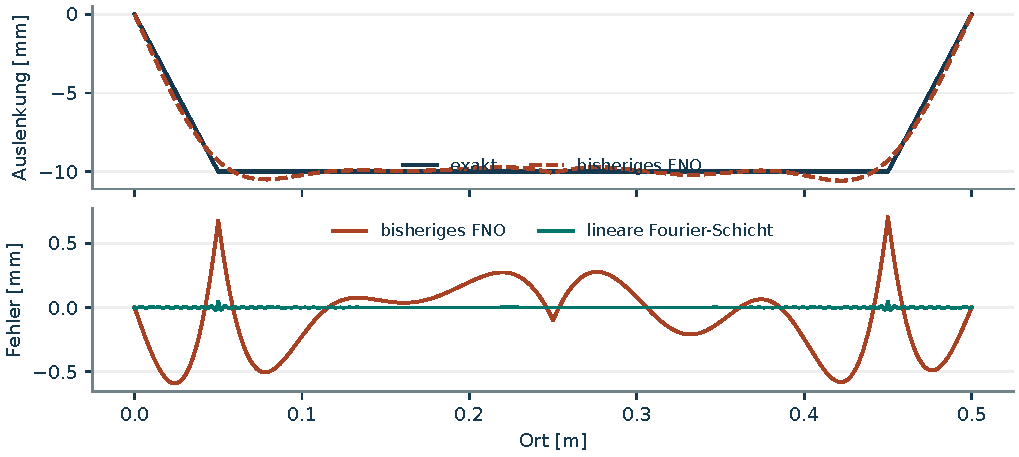
\includegraphics[width=.88\linewidth,height=49mm,keepaspectratio]{fno_saite_feld.pdf}\par}\capline{Das örtliche Fehlerprofil unterscheidet Modelle, die an einem Messpunkt fast übereinstimmen.}
\seite{}{Scientific Machine Learning}\anchorpage{2}{abs9-1}{9.1 · Surrogate, Residuen und Operatoren}\ey{ABSCHNITT 9.1}\ptitle{Surrogate, Residuen und Operatoren}
\hypertarget{punkt9-1-1}{}\subt{9.1.1\enspace Was bildet das Modell ab?}
Ein gewöhnliches Surrogat kann etwa die maximale Auslenkung aus einer einzigen Zugposition schätzen. Bei einer Feldvorhersage sind Eingabe und Ausgabe dagegen ganze Funktionen. Die Messorte, die Norm und die Verteilung der Trainingseingaben legen fest, welche Unterschiede im Lernverfahren überhaupt sichtbar werden.
\hypertarget{punkt9-1-2}{}\subt{9.1.2\enspace Physikalisch informierte neuronale Netze}
Ein PINN setzt eine differenzierbare Netzfunktion in die Differentialgleichung ein. Der Verlust kombiniert PDE-Residuen an Kollokationspunkten mit Anfangs-, Rand- und gegebenenfalls Messfehlern. Eine nahezu konstante falsche Lösung der Wärmegleichung kann einen kleinen inneren Defekt haben, während sie die Randwerte verfehlt. Auch starke Gewichtung einzelner Terme ersetzt keine unabhängige Prüfung zwischen Messpunkten.
\hypertarget{punkt9-1-3}{}\subt{9.1.3\enspace DeepONet und FNO}
Ein DeepONet verknüpft typischerweise Merkmale der Eingabefunktion aus einem Zweignetz mit Ortsmerkmalen eines zweiten Netzes. Ein FNO mischt räumliche Information über spektrale Operatoren. Beide approximieren eine Abbildung zwischen Funktionenräumen auf endlich vielen Beispielen. Ein Test auf neuen Eingabefamilien verlangt eine eigene Stichprobe.
\lektion{Wie lernt ein einzelnes Neuron?}{nnrechnen}{Einstieg}{Neuronale Netze}
\lernziel{Sie können eine Vorhersage, einen Fehler und eine Gewichtsänderung selbst berechnen.}
Stellen Sie sich einen normierten Sensor vor. Für den Eingang \(x=2\) wurde als Ziel \(y=1\) gemessen. Ein künstliches Neuron bildet eine gewichtete Summe und wendet eine Funktion darauf an. Wir verwenden \(\hat y=\max(0,wx)\). Die Funktion \(\max(0,z)\) heißt \emph{ReLU}. Zur ersten Handrechnung setzen wir die sonst häufig verwendete additive Verschiebung auf null.
\subt{Vorhersagen und bewerten}
Wir starten bei \(w=1\). Die Vorhersage ist \(\hat y=2\). Als Verlust dient die Hälfte des quadratischen Fehlers \(L(w)=\tfrac12(\hat y-y)^2\), hier also \(0{,}5\). Der Verlust misst an diesem Trainingsbeispiel, wie gut das Gewicht passt.
\subt{Ein Schritt, der den Verlust verkleinert}
Auf dem positiven Ast der ReLU ist \(\hat y=wx\). Nach der Kettenregel ist \(L'(w)=(wx-y)x=2\). Mit Lernrate \(\eta=0{,}1\) geht der Gradientenabstieg entgegen der positiven Ableitung:
\[
 w_{\rm neu}=w-\eta L'(w)=0{,}8,\qquad
 \hat y_{\rm neu}=1{,}6,\qquad L(w_{\rm neu})=0{,}18 .
\]
Ein Netz verknüpft viele solcher Einheiten zu Schichten. Beim Training werden die Ableitungen mit der Kettenregel von der Ausgabe zurück zu den Gewichten gerechnet (Backpropagation). In der Vorhersage bleiben die gewählten Gewichte fest. Ob das Modell für andere Eingaben taugt, wird an zurückgehaltenen Beispielen geprüft.
\notebox{Eine eigene Gegenprobe}{Bei \(x=-2\) wäre für die Regel \(y=x/2\) das Ziel \(-1\). Die ReLU am Ausgang kann nur Werte ab null liefern. Für eine schwingende Saite muss die Netzausgabe beide Vorzeichen zulassen. Für den Betrag einer Strömungsgeschwindigkeit passt eine nichtnegative Ausgabe.}
\srcs{\texttt{python methodenlabor.py} · \see{pyfno}{Von einzelnen Zahlen zu ganzen Feldern} · \see{netzarten}{Drei Arten, Physik und Lernen zu verbinden}.}

\lektion{PINN, DeepONet oder Fourier-Operator?}{netzarten}{Methodenwahl}{Neuronale Verfahren}
Bei der Saite kann man zwei verschiedene Fragen stellen. Wie schwingt \emph{diese} Anfangsform? Wie ändern sich die späteren Profile, wenn wir die Anfangsform austauschen? Der Auftrag bestimmt die Eingaben eines Netzes und die Information, aus der es lernt.
\subt{Ein physikinformiertes Netz für eine feste Saite}
Ein Physics-Informed Neural Network (PINN) bekommt hier Ort und Zeit und gibt \(u_\theta(x,t)\) aus. Wir bewerten an ausgewählten Punkten den Gleichungsrest \(r=u_{\theta,tt}-c^2u_{\theta,xx}\). Automatische Differentiation leitet dafür die im Netz ausgeführten Operationen ab. In den Verlust gehen außerdem die Fehler bei Anfangsauslenkung, Anfangsgeschwindigkeit und Randwerten ein. Die Nullfunktion hat überall Rest null und erfüllt die festen Ränder. Für eine ausgelenkte Saite verfehlt sie die Anfangsform. Dieser Gegenversuch erklärt, warum die einzelnen Verlustanteile nötig sind.
\subt{DeepONet lernt aus einer Familie von Anfangsformen}
Ein Teilnetz liest Messwerte der Eingabefunktion \(g\) an festgelegten Sensororten und liefert Koeffizienten \(b_k(g)\). Ein zweites Teilnetz liest den abzufragenden Ort und die Zeit und liefert Basiswerte \(t_k(x,t)\). Ihre Summe von Produkten \(\sum_k b_k(g)t_k(x,t)\) gibt die Vorhersage. Für die Familie \(g(x)=a\sin(\pi x/L)\) genügt ein Produkt bereits exakt: Der Mittensensor liefert \(a\), der zweite Faktor ist \(\sin(\pi x/L)\cos(\pi ct/L)\). Gegenaufgabe bei \(t=0\): Vergleichen Sie \(g_1=0\) mit \(g_2=a\sin(2\pi x/L)\), \(a\ne0\). Am Mittensensor liefern beide null. Bei \(L/4\) liefern sie 0 bzw. \(a\). Gleiche Sensoreingaben können daher verschiedene Ausgaben verlangen.
\subt{FNO liefert im CP2-Versuch ganze Gitterprofile}
Unser FNO bekommt das Eingabefeld auf dem Gitter. Es mischt räumliche Frequenzen und lokale Merkmale. Die Trainingsziele stammen für die Saite aus der Modenlösung und für die Kavität aus dem D2Q9-Code. PINN und DeepONet sind hier Entwurfsalternativen. Die gemessenen CP2-Netzfehler gelten für das tatsächlich trainierte FNO.
\srcs{\href{https://doi.org/10.1016/j.jcp.2018.10.045}{Raissi u.\,a. (2019), PINNs} · \href{https://www.nature.com/articles/s42256-021-00302-5}{Lu u.\,a. (2021), DeepONet} · \see{pyvergleich}{Gemessene FNO-Fehler}.}

\seite{}{Scientific Machine Learning}\anchorpage{2}{abs9-2}{9.2 · Eine Fourier-Neural-Operator-Schicht}\ey{ABSCHNITT 9.2}\ptitle{Eine Fourier-Neural-Operator-Schicht}
\hypertarget{punkt9-2-1}{}\subt{9.2.1\enspace Eine Faltung über das ganze Feld}
Für einen translationsinvarianten Kern \(k(x-y)\) ist die Faltung \(\int k(x-y)v(y)\,dy\) im periodischen Fall im Fourierraum eine Multiplikation. Eine tiefe Operatorarchitektur lernt diesen globalen Anteil und kann über einen lokalen Term und Nichtlinearitäten komplexere Abbildungen darstellen.
\hypertarget{punkt9-2-2}{}\subt{9.2.2\enspace Von der FFT zurück in den Ortsraum}
Eine Schicht berechnet \(v^+=\sigma(Wv+b+\mathcal F^{-1}(R_k\widehat v_k))\). Zuerst transformiert die FFT jeden Eingangskanal. Für die behaltenen Moden mischt die komplexe Matrix \(R_k\) die Kanäle. Andere Moden des spektralen Zweigs werden auf null gesetzt. Nach der inversen FFT addiert man die punktweise affine Abbildung. Für ein reelles Feld müssen die Fourierkoeffizienten die konjugierte Symmetrie erfüllen. Zeichnen Sie die zwei parallelen Wege und markieren Sie den einzigen Schritt, der über alle Orte koppelt.
\hypertarget{punkt9-2-3}{}\subt{9.2.3\enspace Übertragung auf ein feineres Gitter}
Dieselben Gewichte können auf kompatiblen Gittern dieselben physikalischen Moden ansprechen. Dafür müssen Intervall, Randbehandlung, Normierung und Modenzuordnung passen. Ein auf einem groben Gitter unaufgelöster Knick bleibt eine Herausforderung. Der Test vergleicht dieselbe Eingangsfunktion auf zwei Gittern gegen eine unabhängige Lösung und nennt für jedes Gitter den Feldfehler.
\srcs{\href{https://arxiv.org/abs/2010.08895}{Li und andere, Fourier Neural Operator} · \see{fnotransfer}{CP2-Gitterwechsel}.}
\lektion{Was lernt ein neuronaler Operator?}{pyfno}{Verfahren}{Neuronale Operatoren}
Ein gewöhnliches künstliches Neuron bildet Eingaben \(z_j\) auf \(a=\sigma(b+\sum_j w_j z_j)\) ab. Die Gewichte \(w_j\) und der Versatz \(b\) werden gelernt. \(\sigma\) ist eine vorgegebene, gewöhnlich nichtlineare Aktivierungsfunktion. Ein \emph{Operator} ordnet hier einer ganzen Eingabefunktion eine oder mehrere Ausgabefunktionen zu. An einem Gitter sehen wir diese Funktionen als Zahlenfelder.
\subt{Eine Schicht des Fourier Neural Operator}
Ein FNO zerlegt seine internen Felder mit einer diskreten Fouriertransformation in räumliche Frequenzen. Für ausgewählte Frequenzen mischt er die Merkmale mit lernbaren Matrizen. Nach der Rücktransformation addiert er einen lokalen Beitrag und wendet eine Aktivierung an. Aus mehreren solchen Schichten entsteht in der Saite die Abbildung \(g(\cdot)\mapsto (u(\cdot,5),u(\cdot,8))\). Die analytische Kontrollrechnung verwendet bekannte Wellengesetze; die Matrizen des Netzes werden an Beispielen bestimmt.
\subt{Woher kommen richtige Trainingsantworten?}
Für die Saite ziehen wir unabhängige Anfangsprofile aus acht Sinusmoden. Die \(k\)-te Mode wird mit \(\cos(k\pi ct/L)\) multipliziert. Für die Kavität variieren wir die anfängliche Dichte sanft um eins, bei ruhender Flüssigkeit und gleichem Deckel. Für jedes Eingabefeld erzeugt D2Q9 das Ziel \(|\mathbf u|/u_\mathrm{Deckel}\). Ein Betrag am Netzausgang erzwingt nichtnegative Vorhersagen. Bei der Saite erzwingt eine ungerade Projektion verschwindende Randwerte.
\subt{Welche Daten darf das Netz sehen?}
Je Fall dienen 96 ganze Felder zum Optimieren der Gewichte. Nach jeder Epoche bewerten wir 16 weitere Felder und speichern die besten Gewichte. Erst danach werten wir 24 andere Felder aus. Bei der Saite kommen Dreiecksform und feineres Gitter als zusätzlicher Transfer hinzu, bei der Kavität der gleichförmige Ruhezustand. Eine Aufteilung einzelner Gitterpunkte derselben Trajektorie könnte dasselbe Experiment in beiden Mengen erscheinen lassen.
\srcs{\href{https://github.com/neuraloperator/neuraloperator}{NeuralOperator, Python-Paket neuraloperator} · \href{https://openreview.net/pdf?id=c8P9NQVtmnO}{Li u.\,a. (2021), Fourier Neural Operator} · \cpcode{argesim_benchmarks/experiments/cp2_fields.py}{Erzeugung der Referenzfelder}.}

\lektion{Saite · Wie lernt eine Fourier-Schicht?}{fnosaite}{Labor}{CP2 · Saite}
Denken Sie sich die gezupfte Saite aus einfachen Schwingungsformen zusammengesetzt. Die \(k\)-te Form \(\sin(k\pi x/L)\) verschwindet an beiden Enden. Bei einer idealen linearen Saite bleibt jede Form für sich erhalten; nur ihre Amplitude ändert sich. Ein trainierbarer Faktor \(m_k(t)\) pro Mode genügt daher. Wie groß er sein soll, lernt die Fourier-Schicht aus Paaren von Eingangs- und Ausgangsamplituden.
\[
 \widehat m_k(t_i)=
 \frac{\sum_j a_{jk}(0)\,a_{jk}(t_i)}{\sum_j a_{jk}(0)^2}.
\]
Mit angeregter Mode folgt die Formel aus der Ableitung der Fehlerquadratsumme. Die 96 Profile liefern Faktoren für 192 Moden und 321 Zeiten von 0 bis 8 s. Dazwischen interpolieren wir linear. Für die Referenz gilt \(m_k(t)=\cos(ck\pi t/L)\). Setzt man \(a_{jk}(t_i)=a_{jk}(0)\cos(\omega_kt_i)\) ein, kürzt sich die Summe der Quadrate. Im Kontrolllauf ersetzen wir nur die Faktoren durch diesen Kosinus, bei gleicher Modenzahl und Interpolation. Die Sinustransformation entspricht der Fourier-Transformation der ungeraden Fortsetzung.
\minifig{fno_saite_feld}{59mm}{Mittig gezupfte Saite auf 501 Knoten. Oben stehen die Profile für 5 und 8 s, unten die lokalen Fehler auf derselben Millimeterskala. Das ursprüngliche FNO glättet die Knicke.}
\subt{Der Vergleich am selben Dreieck}
Nach 5 s fällt der relative Fehler von \(3{,}0009\,\%\) auf \(0{,}04303\,\%\), nach 8 s von \(0{,}8816\,\%\) auf \(0{,}01416\,\%\). Die analytische Kontrollschicht erzielt ebenfalls \(0{,}04303\,\%\) und \(0{,}01416\,\%\). Ihr größter Profilabstand zur gelernten Schicht liegt unter \(5\cdot10^{-14}\unitm m\). Der neue absolute RMS beträgt \(4{,}00\) bzw. \(4{,}05\,\mu\mathrm m\). Newmark erreicht \(0{,}3745\) bzw. \(0{,}1519\,\%\), Störmer--Verlet \(0{,}2313\) bzw. \(0{,}0946\,\%\) bei den Einstellungen der vorangehenden Studie.
\srcs{Eine Auswertung derselben Gewichte mit \href{https://neuraloperator.github.io/dev/modules/generated/neuralop.layers.spectral_convolution.SpectralConv.html}{NeuralOperator · SpectralConv} unterscheidet sich hier um höchstens \(1{,}23\cdot10^{-8}\unitm m\) von der Sinusauswertung.}

\lektion{Welche Fehlergrenze lässt sich beweisen?}{fnobeweis}{Vertiefung}{CP2 · Operatortheorie}
Schreiben wir die Anfangsform in einer orthonormalen Sinusbasis als \(g=\sum_k a_k e_k\). Orthogonalität bedeutet hier \(\|g\|_2^2=\sum_k |a_k|^2\). Eine präzise Annahme an die Glattheit lautet \(\sum k^{2s}|a_k|^2\le R^2\), \(s>0\). Große \(s\) begrenzen die Energie schneller räumlicher Wechsel stärker.
\subt{Satz für die trainierte lineare Schicht}
Seien \(K\) die behaltenen Moden, \(\omega_k=ck\pi/L\), \(d\) der größte Abstand zweier Zeitstützstellen und \(\epsilon\) der größte Fehler eines gespeicherten Faktors an einer Stützstelle. Für \(0\le t\le8\) gilt
\[
 \|(\widehat S(t)-S(t))g\|_2 \le R\max\!\left\{
 \max_{1\le k\le K}\frac{\epsilon+\omega_k^2d^2/8}{k^s},
 (K+1)^{-s}\right\}.
\]
\proofpart{Der Fehler linearer Interpolation einer zweimal differenzierbaren Funktion ist höchstens \(d^2\max|m''|/8\). Für den Kosinus ist \(\max|m_k''|\le\omega_k^2\); ein konvexes Mittel zweier Stützfehler hat Betrag höchstens \(\epsilon\). Ab Mode \(K+1\) ist der Betrag des ausgelassenen Multiplikators höchstens eins. Quadrieren, in der orthonormalen Basis summieren und den größten gewichteten Faktor ausklammern liefert die Behauptung.}
Eine Intervallauswertung aller 61\,632 gespeicherten Faktoren ergibt \(\epsilon<1{,}36\cdot10^{-13}\). An den Stützzeiten entfällt der Interpolationsterm. Auf einem festen Gitter gilt die Rechnung für dessen diskrete Sinuskoeffizienten mit \(K\le N-2\). Bei einer abgetasteten kontinuierlichen Form kommt der Fehler ihrer räumlichen Darstellung hinzu. Die Gitterstudie misst ihn mit.
\subt{Was lässt sich über das frühere mehrschichtige FNO sagen?}
Für das frühere Netz liefert die Verkettung von Schichtnormen \(\|F(g)-F(h)\|_2\le24\,217\|g-h\|_2\). Jede Fourier-Matrix wird durch ihre Frobeniusnorm beschränkt, die GELU-Ableitung durch \(1{,}13\); bei parallelen Zweigen addieren sich Grenzen. Ungerade Projektion macht \(F(0)=0\). Für jede einzelne Ausgabe und eine diskrete Eingabekugel mit Radius \(R\) folgt so \(24\,218R\) als konservative absolute Fehlergrenze. Die genauere modale Schranke oben nutzt wesentlich mehr Modellstruktur.
\srcs{\texttt{scripts/cp2\_accuracy/operator\_bounds.py} prüft die festen binären Gewichte als reelle Koeffizienten mit nach außen gerundeter Intervallarithmetik. Die Laufzeitrundung einer GPU ist eine eigene Fehlerquelle.}

\seite{}{Scientific Machine Learning}\anchorpage{2}{abs9-3}{9.3 · Physikalischer Basissolver und gelernte Korrektur}\ey{ABSCHNITT 9.3}\ptitle{Physikalischer Basissolver und gelernte Korrektur}
\hypertarget{punkt9-3-1}{}\subt{9.3.1\enspace Welchen Anteil übernimmt das Netz?}
Für eine grobe Vorhersage \(B(a)\) und eine feine Referenz \(G(a)\) kann das Lernziel \(G(a)-B(a)\) sein. Dann ergibt sich \(\hat G=B+N_\theta\). Ein sauberes Experiment enthält den unveränderten Basissolver, eine analytische Korrektur, soweit vorhanden, und die Netzkorrektur auf identischen Testfeldern. So wird bei der Saite sichtbar, was bereits die Modenwahl und die Randfortsetzung leisten.
\hypertarget{punkt9-3-2}{}\subt{9.3.2\enspace Fehlertransport und Verallgemeinerung}
Wird ein gelernter Einzelschritt immer wieder eingesetzt, kann sich ein Defekt \(\delta\) unter einer Lipschitz-Schranke \(K\) zu \(\|e_n\|\le K^n\|e_0\|+\delta\sum_{j=0}^{n-1}K^j\) aufsummieren. Eine direkte Vorhersage zu einem festen Endzeitpunkt hat einen anderen Fehlerweg. In CP2 prüfen gespiegelte Zupfstellen die Symmetrie. Eine neue Reynolds-Zahl der Kavität prüft dagegen den Transfer auf einen anderen Betriebspunkt.
\notebox{Gegenprobe}{Teilen Sie die Testdaten nach physikalischer Eingabefamilie. Werden Nachbarn derselben Trajektorie auf Training und Test verteilt, beantwortet der gemessene Fehler eine wesentlich leichtere Frage.}
\lektion{Was ist beim Methodenvergleich noch offen?}{forschungsmethoden}{Forschung}{Methodenvergleich · November 2026}
\subt{Klassische Diskretisierung und Lattice-Boltzmann}
Am Transportbeispiel lassen sich Erhaltung, Positivität und Genauigkeit einzeln testen. Für die CP2-Saite ist die Schrittgrenze der expliziten Diskretisierung herleitbar. Der Gitterversuch für die Fourier-Schicht vergleicht die geknickte Saite bereits an \(6\cdot4\cdot99=2\,376\) Kombinationen aus Zupfposition, Gitter und Zeit (S.\,\pagelink{fnoabl}). Offen bleibt das genaue kontinuierliche Maximum des absoluten RMS-Fehlers für diese Dreiecke auf \([0,8]\unitm s\). Die Schranke auf S.\,\pagelink{fnobeweis} gilt unter ihren dort angegebenen Regularitätsannahmen.

Eine Untersuchung von LBM-Randregeln aus dem Jahr 2024 vergleicht Varianten an laminaren Strömungen mit bekannten Referenzen. Das ist für CP2 wichtig, weil unser Deckel seine Geschwindigkeit vorschreibt. Für die stationäre Kavität publizierten Ghia, Ghia und Shin Vergleichsdaten. Der \see{fnolang}{vollständige Kavitätslauf} prüft inzwischen beide Geschwindigkeitskomponenten, die Annäherung an den stationären Zustand und drei Gitterweiten.
\subt{Was zeigt die Forschung zu gelernten Operatoren?}
Herde u.\,a. untersuchten 2024 mit Poseidon ein vortrainiertes Modell an 15 nachgelagerten PDE-Aufgaben. Park u.\,a. verglichen 2026 in einem Preprint kurze und lange Vorhersagefolgen mehrerer Modelle. In ihrer Untersuchung wuchs der Fehler bei vielen längeren Folgen. Beide Studien betreffen andere Daten und Architekturen als unser CP2-Praktikum.
\subt{Wie groß ist der Gewinn auf unabhängigen Daten?}
Die anschließende Studie prüft sechs Zupfpositionen, absolute und relative Fehler sowie veränderte Deckelgeschwindigkeiten, Zeitschritte und Gitter. Zwei Rechnungen zeigen, welcher Anteil der Verbesserung von der Modellstruktur und welcher vom neuronalen Anteil stammt. Eine bewiesene Fehlergrenze nutzt die lineare Wellengleichung.
\srcs{\href{https://doi.org/10.1016/j.camwa.2024.08.009}{LBM-Randbedingungen (2024)} · \href{https://doi.org/10.1016/0021-9991(82)90058-4}{Ghia u.\,a. (1982)} · \href{https://proceedings.nips.cc/paper_files/paper/2024/hash/84e1b1ec17bb11c57234e96433022a9a-Abstract-Conference.html}{Herde u.\,a. (NeurIPS 2024)} · \href{https://arxiv.org/abs/2610.31935}{Park u.\,a. (Preprint, Oktober 2026)}.}

\lektion{Eine Spektralschicht ohne verdeckte Achsen}{alg9}{Werkstatt}{Kapitel 9}
Wir nehmen ein reelles Eingangsfeld mit einer Kanalachse und einer räumlichen Achse. Für diesen Lehrschritt ist die Länge N fest, und K überschreitet die Zahl der verfügbaren reellen FFT-Moden nicht. Randfortsetzung und Normierung müssen schon zur Datenerzeugung passen.
{\small\begin{verbatim}
v_hat = rfft(v, axis=Ort)
z_hat = komplexe_Nullen(Ausgabekanaele, N//2 + 1)
fuer k in den ersten K Moden:
    z_hat[:,k] = R[k] @ v_hat[:,k]
spektral = irfft(z_hat, n=N, axis=Ort)
v_neu = Aktivierung(spektral + W @ v + bias)
\end{verbatim}}
\subt{Selbst rechnen}
Ein Eingang enthält nur eine Mode oberhalb der behaltenen K Moden. Was kann dieser einzelne lineare spektrale Pfad übertragen?
\notebox{Lösung}{In diesem Pfad ist die Ausgabe null. Der lokale Pfad W kann den Eingang trotzdem weiterreichen. Nach einer Nichtlinearität können zusätzliche Frequenzen entstehen. Deshalb belegt die Modenabschneidung eines Zweiges allein keine Bandbegrenzung des gesamten Netzes.}
\bilanz{I}{Von der Modellfrage zur zulässigen Solverform}{finalI}
\subt{Stand der Forschung im Zusammenhang}
Die klassische Theorie der Anfangswertprobleme liefert klare Aussagen über umgeformte ODEs. Forschung zur symbolischen Indexreduktion und zur Schrittsteuerung behandelt zwei nachgelagerte Schwierigkeiten: das Erkennen verborgener Bindungen und das zuverlässige Einhalten eines Fehlerziels. Bei hybriden Übergängen kommt die Lokalisierung der Ereigniszeit hinzu. Die drei Aufgaben benutzen unterschiedliche Voraussetzungen.
{\tblstart\begin{tabularx}{\linewidth}{@{}P{34mm}YY@{}}\toprule
\hd{Operation}&\hd{Was im Buch bewiesen ist}&\hd{Welche Bedingung entscheidet}\\\midrule
\(q^{(n)}\) umformen&Eins-zu-eins-Zuordnung der glatten Lösungen.&Die höchste Ableitung ist auf dem gewählten Zweig bestimmbar.\\
Algebraik eliminieren&Lokale Rekonstruktion bei regulärem Index 1, identische diskrete RC-Rechnung.&Konsistenter Start und invertierbares \(g_z\).\\
Ort diskretisieren&Diskretes Maximumprinzip der Diffusion und Stabilitätsgrenze.&Gitter, Zeitschritt, Randdaten und Vorzeichen der Gewichte.\\
Ereignis lokalisieren&Zeitfehler höchstens Wächterfehler dividiert durch Mindeststeigung.&Wahre einfache Nullstelle im betrachteten Intervall.\\\bottomrule\end{tabularx}\par}
\subt{Ein offener Nachweis als Brücke zum Labor}
Kombiniert man eine räumlich diskretisierte PDE, eine algebraische Randbedingung und einen schaltenden Regler, reicht keiner der Einzelsätze für eine Gesamtgarantie. Erforderlich wären gemeinsame Schranken für die Semidiskretisierung und die algebraische Lösung sowie ein von null getrennter Nulldurchgang. Im Praktikum untersuchen wir diese Mechanismen an getrennten Fällen. Ein Beweis für ihre volle Kopplung bleibt eine klar abgegrenzte Erweiterung.
\srcs{\see{schluss2}{Ordnungsreduktion} · \see{schluss4}{Schrittsteuerung} · \see{schluss5}{DAE} · \see{schluss6}{Gitter} · \see{schluss7}{Ereigniszeit}.}
